\section{Implementierung}
\label{sec:implementierung}
Nachdem die Anforderungsanalyse beendet, und die Ziele bestimmt wurden, wurden alle Funktionalitäten implementiert. Dabei wurde in Richtung Front-End zu Back-End gearbeitet. Diese Reihenfolge wird auch im folgenden Kapitel eingehalten. Zum einem um den Entwicklungsprozess wieder zu spiegeln, zum anderen um die Gedankengänge besser darzustellen, die sich durch die Entwicklungsreihenfolge entwickelt haben.

\subsection{Client - Darstellung}
\label{subsec04:client_viz}
In dem ersten Abschnitt wird die Entwicklung des Clients beschrieben. Dieser dient letzten Endes zu der Bedienung und Darstellung der Software. Neben der Funktionalität, muss zusätzlich auf Bedienbarkeit und Verständlichkeit der Software geachtet werden.

\subsubsection{Informationen vom Server}
\label{subsubsec04:info_server}

In der schon bereits vorhandenen Software gibt es eine erste Implementierung, die die Informationen vom Server an den Client sendet.
Der Client speichert diese Informationen in einem ``Interface'' (siehe: Listing~\ref{lst:desc_schema}). 

\lstinputlisting[
  language=javascript,
  caption=Interface einer Tabelle und Spalte,
  label=lst:desc_schema,
  float=h,
  numbers=left
]{snippets/schema.description.ts}

Eines der Grundprinzipien von Typescript, ist die Typprüfung. Interfaces erfüllen dabei die Rolle der Benennung der Typen und bestimmen Schnittstellen innerhalb des Projektes und zum Code außerhalb.~\cite{typescript_interfaces}

Damit ist festgeschrieben welche Eigenschaften eine Tabelle und die dazugehörigen Spalten besitzen müssen. Bis zu diesem Zeitpunkt wurden die Informationen der Datenbank, nur verwendet um diese, beim Erstellen von SQL-Statements, auszuwählen. Mit der dazu kommenden Funktionalität der Migration, werden Funktionen auf einzelne Tabellen oder Spalten angewendet. Diese Funktionen lassen sich nicht in einem Interface abspeichern. Für eine leichtere Anwendung und der Verhinderung globale Funktionen zu definieren, wurden zwei Klassen implementiert. In einer Tabellen und Spalten Klasse konnten die einzelnen Funktionen für die weitere Implementierung programmiert werden.


\subsubsection{Fehlende Foreign Keys}
\label{subsubsec04:miss_fk}

Bei der Analyse der Daten die vom Server versendet werden (siehe: Listing~\ref{lst:desc_schema}), wurde festgestellt, dass die Foreign Keys der einzelnen Tabellen nicht übermittelt wurden.
Für die akkurate Darstellung des Schemas sind die Foreign Keys der einzelnen Tabellen notwendig, um die einzelnen Relationen anzeigen zu können.
Dafür mussten die Informationen zuerst von der Datenbank erfragt und dann versendet werden (siehe dafür:~\ref{subsubsec04:fk_table_server}).
Da im Gegensatz zu Tabellen und Spalten keine direkten Veränderungen an Foreign Keys möglich sind, sondern nur das Hinzufügen und Entfernen dieser, müssen diese nicht in einer eigenen Klasse abgebildet werden.

\lstinputlisting[
  language=javascript,
  caption=Interface: Foreign Keys,
  label=lst:fk,
  float=h,
  numbers=left
]{snippets/foreign_key.description.ts}

\subsubsection{Anzeige des Schemas}
\label{subsubsec04:anz_schema}

Die Darstellung des Schemas ist der Einstiegspunkt der Komponente und soll neben der Darstellung auch die Bedienung und Weiterleitung zu den weiteren Funktionen liefern.

\begin{description}
\item[Angular 2] \hfill\\
Im ersten Schritt wurden die Daten, die vom Server zur Verfügung gestellt wurden, in simpler Art auf dem Bildschirm dargestellt. 
Dafür bietet Angular 2 ``Templates'' an. Templates definieren damit das Aussehen einer Komponente. Templates sehen dabei aus wie \texttt{HTML}-Dokumente, mit ein paar Unterschieden~\cite{angular2_flow}.

\begin{figure}[ht]
    \frame{\includegraphics[width=\textwidth]{images/kap-4-angular2_overview.png}}
    \centering
    \caption{Angular 2 Architektur}
    \label{pic:angular2_architecture}
\end{figure}

Bei diesen Unterschieden handelt es sich um Erweiterungen, die bestimmte Funktionalitäten zu dem \texttt{HTML} Standard hinzufügen. Die wichtigsten und in diesem Projekt am häufigsten angewandten Erweiterungen sind folgende:
\begin{itemize}
\item Direkter Zugriff auf Variablen einer Komponente (Property Binding)
\item Funktionen direkt an Events zu verknüpfen (Event Binding)
\item If-Anweisungen 
\item Schleifen
\end{itemize} 


\item[Bootstrap] \hfill\\
Bootstrap ist ein \texttt{CSS}-Framework, welches in dem Projekt bereits eingebunden ist. Damit lassen sich auf schnelle und einfache Art \texttt{HTML}-Dokumente gestalten. 
Eines der in Bootstrap vorhandenen Gestaltungsvorlagen sind die ``Cards''\footnote{\url{https://v4-alpha.getbootstrap.com/components/card/}}, die für die Gestaltung der einzelnen Tabellen benutzt wurde.

\begin{figure}[ht]
    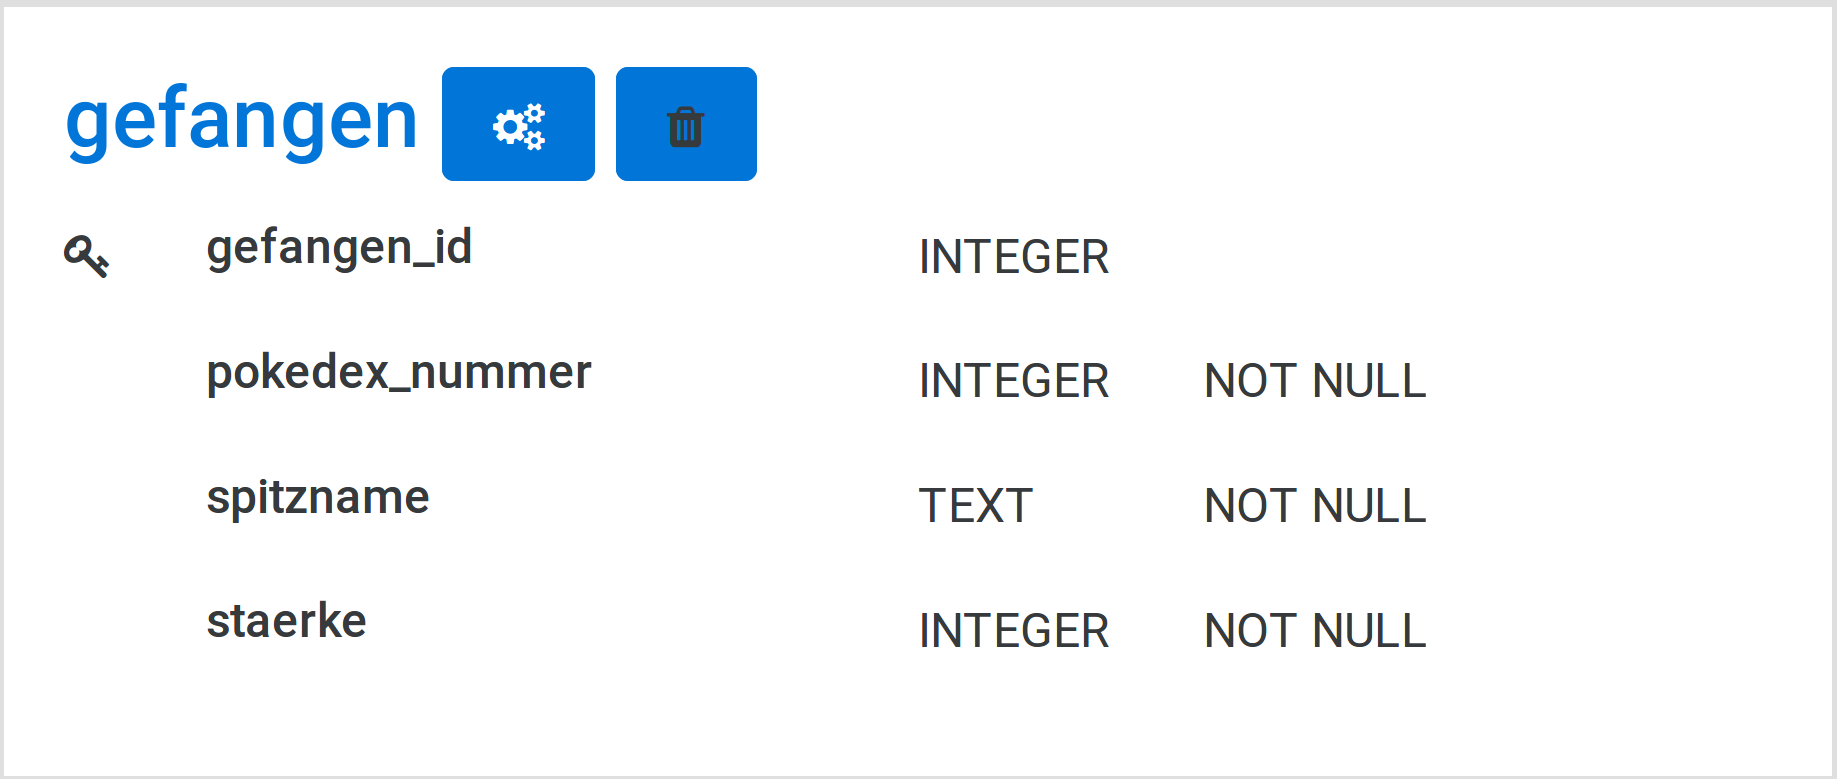
\includegraphics[width=\textwidth]{images/kap-4-tableView.png}
    \centering
    \caption{Darstellung einer Tabelle mit Bootstrap}
    \label{pic:table_boot}
\end{figure}

\item[Font Awesome] \hfill\\
Um die Darstellung ein wenig angenehmer für die Benutzer zu machen, wurden auf Symbole zurückgegriffen, um einige Informationen in der Tabelle oder Buttons darzustellen. In der ursprünglichen Entwicklung der Software, wurde dafür der Icon-Font\footnote{\url{https://de.wikipedia.org/wiki/Font_(Informationstechnik)}} ``Font Awesome'' eingebunden. Dieser Font wurde unter anderem dann auch zur Visualisierung der Primärschlüssel verwendet.(siehe: Grafik~\ref{pic:table_boot}) 

\item[Graphviz] \hfill\\
Im bereits vorhandenen Server war eine Schnittstelle zu einem Graphviz-Service\footnote{\url{http://www.graphviz.org/}} integriert. Graphviz ist ein Programmpaket um Grafiken darzustellen. Dieses kann dazu verwendet werden, um eine Darstellung des Datenbankschemas zu erzeugen und anzuzeigen. Speziell ermöglicht Graphviz eine weitere Möglichkeit das ganze Schema, mit nur den nötigsten Informationen, auf einen Blick sehen zu können.
Ein Beispiel ist in der Grafik~\ref{pic:graphviz_schema} zu sehen.

\begin{figure}[ht]
    \frame{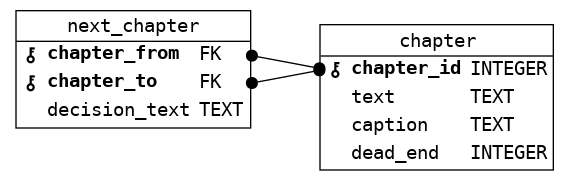
\includegraphics[width=\textwidth]{images/visual_schema.png}}
    \centering
    \caption{Graphviz Schema Darstellung}
    \label{pic:graphviz_schema}
\end{figure}

\item[Zusätzliche Darstellung der Foreign Keys] \hfill\\
Zusätzlich zu der Darstellung mit Graphviz wird, wenn der Benutzer mit dem Mauszeiger über einer Spalte ist, die Tabelle und Spalte eingeblentet, auf die die Spalte verweist. (siehe Grafik:~\ref{pic:table_fk_view})

\begin{figure}[ht]
    \frame{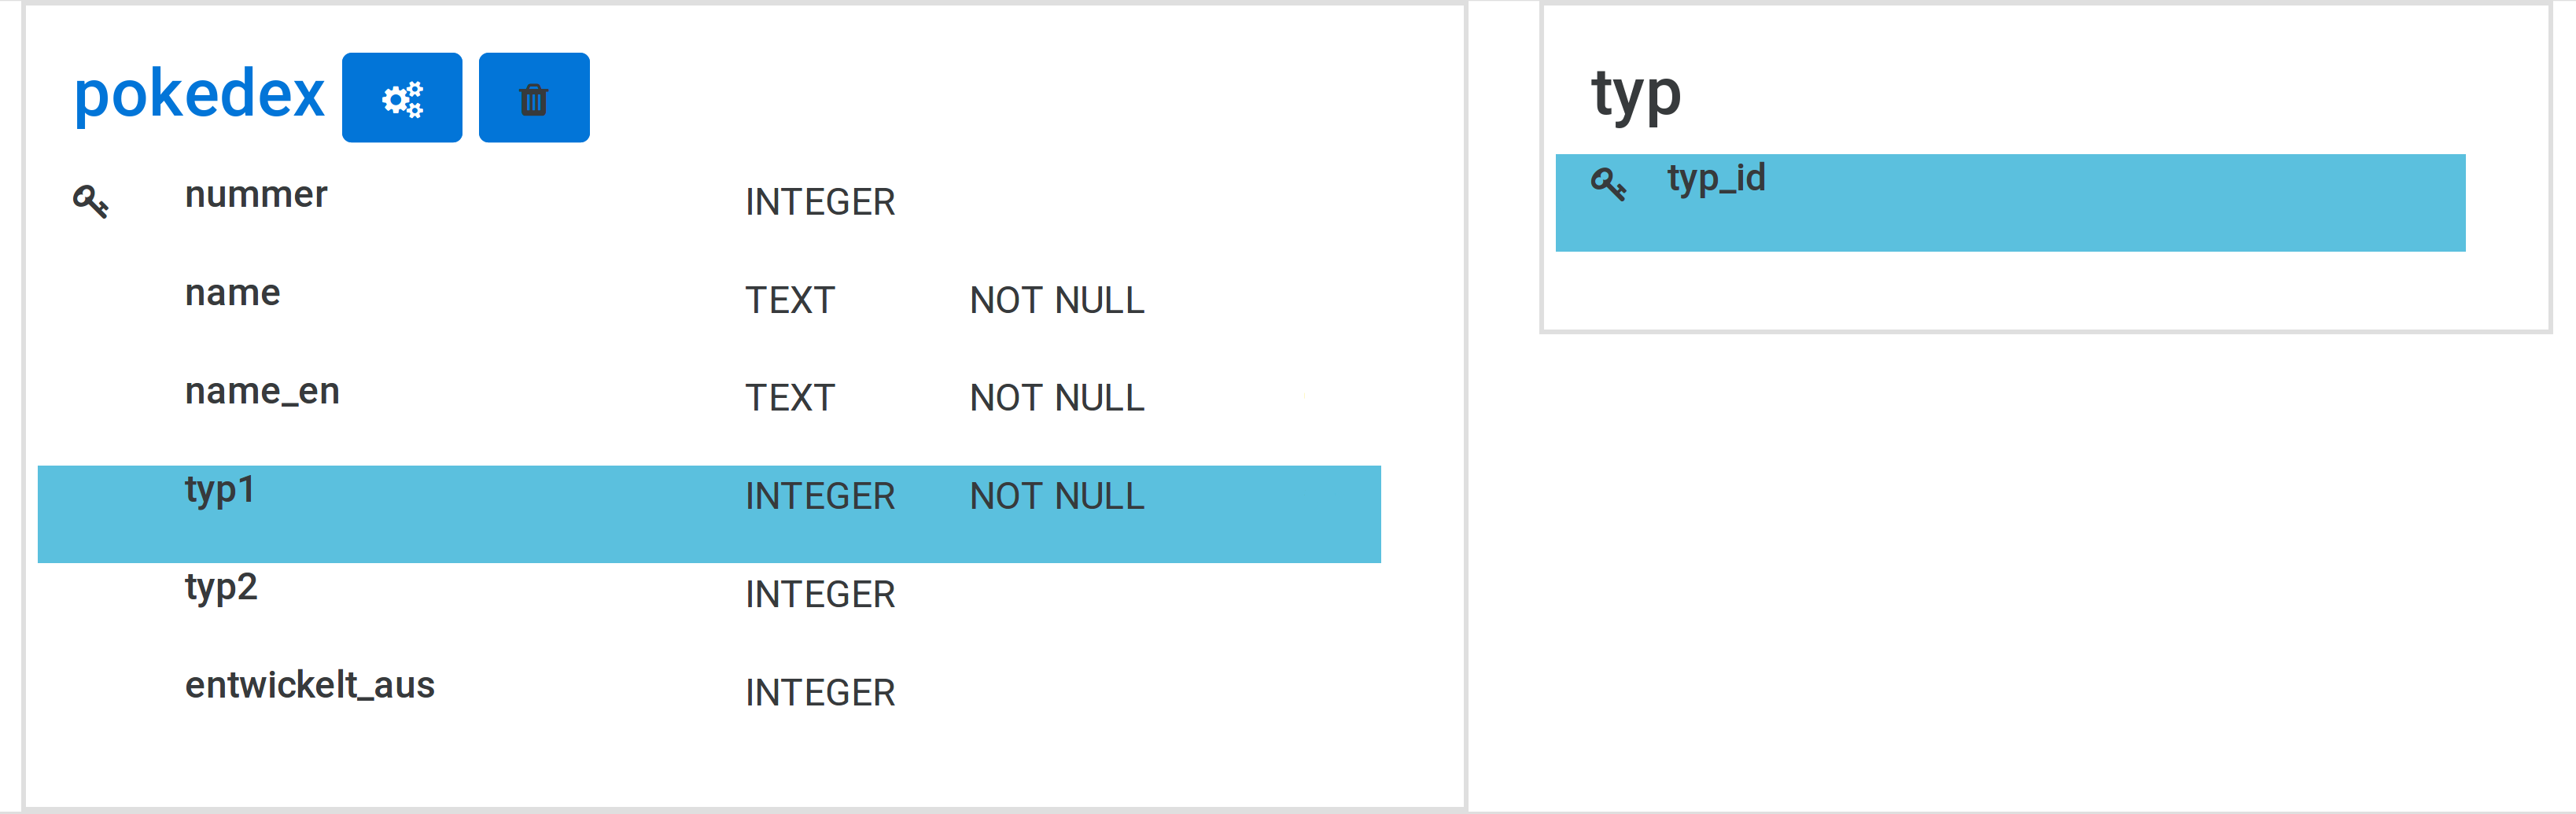
\includegraphics[width=\textwidth]{images/kap-4-table-fk.png}}
    \centering
    \caption{Darstellung eines Foreign Keys}
    \label{pic:table_fk_view}
\end{figure}

\end{description}

\subsubsection{Tabelleninhalte}
\label{subsubsec04:table_content}

In Blattwerkzeug bestand bereits die Möglichkeit SQL-Statements auszuführen. Es ist also möglich eine Abfrage der Art ``\texttt{Select * from \textsc{Tabellenname}}'' auszuführen, und sich damit alle Daten aus einer Tabelle anzeigen zu lassen. In Anbetracht darauf, dass Blatt-werkzeug eine Software zum Erlernen von Datenbanken und deren Umgang ist, soll es möglich sein die Daten einer Tabelle in einer übersichtlichen Ansicht anzeigen zulassen, sowie es in anderen ähnlichen Programmen~\ref{sec02:vergleichbare_arbeiten}, die dieses zur Verfügung stellen, üblich ist.
Die Daten kommen vom Server in ein 2-Dimensionales Array, eine Dimension für jede vorhandene Spalte und die zweite Dimension für die einzelnen Zeilen der Spalte.
In Abschnitt~\ref{subsubsec04:anfragen_darstellung} wird dann im Detail darauf eingegangen, wie die Daten im Server von der Datebbank abgefragt werden.

Ein Beispiel einer solcher Darstellung ist in der Grafik~\ref{pic:table_content} dargestellt.

\begin{figure}[ht]
    \frame{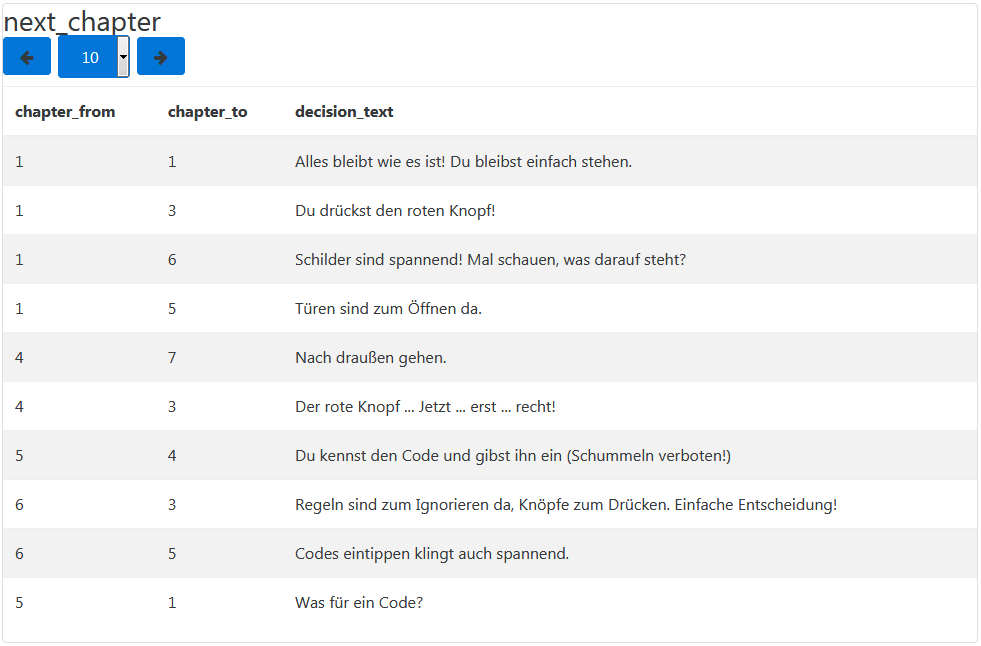
\includegraphics[width=\textwidth]{images/table_content.png}}
    \centering
    \caption{Darstellung der Tabelleninhalte}
    \label{pic:table_content}
\end{figure}

\begin{description}
\item[Verwendung Angular 2 \& Bootstrap] \hfill\\
In der Darstellung der Daten konnte das 2-Dimensionale Array direkt in dem Template der Komponente eingebunden werden. Im folgendem sieht man die Verwendung der Angular 2 Templates mit der zusätzlichen Verwendung von Bootstrap, die im Abschnitt~\ref{subsubsec04:anz_schema} erwähnt wurden.
Dabei ist in Zeile 1 die \texttt{class}-Eigenschaft auf ``table table-striped'' gesetzt um die von Bootstrap zur Verfügung gestellte Tabellendarstellung zu verwenden. Dabei sorgt die zweite \texttt{class}-Eigenschaft, dafür dass die Tabellenzeilen, gestreift angezeigt werden, zur besseren Übersicht.
In den Zeilen 5,13,14 sind von Angular 2 Schleifen zu sehen und in Zeile 6 und 15, dass mit ``Property Binding'' direkt auf eine Variable aus der ``Component'' zugegriffen wird.

\lstinputlisting[
  language=HTML,
  caption=Code zur Darstellung von Tabelleninhalte,
  label=lst:table_entry,
  float=h,
  numbers=left
]{snippets/table_content.ts}

\item[Pagination] \hfill\\
Es ist zu berücksichtigen, dass einige Tabellen gefüllt sein können mit einer großen Datenmenge. Damit ein endlos langes Scrollen verhindert wird und den Datentransfer zwischen Datenbank-Server und Server-Client zu minimieren, wurde eine ``Pagination'' eingebaut. Damit kann die Anzahl an gleichzeitig angezeigten Daten gewählt werden, und mit den Pfeil-Buttons, kann zwischen den Pages~\footnote{Seiten - hier Satz an Daten} geschaltet werden. 

\end{description}

\newpage

\subsection{Client - Editor}
\label{subsec04:client_edit}

Im folgendem Kapitel soll die Implementierung des Editors auf Clientsseite erklärt werden. Dieser und der korrespondierende serverseitige Abschnitt werden deutlich und ausführlich behandelt, da es der Kern dieser Ausarbeitung ist.
Die Migration eines Schemas einer Datenbank, ist im Allgemeinen das Verändern der Datenbank, mit der Absicht diese auf neue Gegebenheiten anzupassen oder zu erweitern. Zusätzlich ist im allgemeinen Sinne der Migration, auch die Möglichkeit gegeben, das Schema auf eine ältere Version zurückzuführen.
In Anbetracht der hier vorliegenden Software, wird nur die Möglichkeit geboten das Schema anzupassen, ohne einer Versionskontrolle.
Da die Thematik der Schemamigration ein sehr komplexes ist, mit möglichen ir­re­ver­si­blen Fehlern, wird hier eine ausführliche Erklärung gegeben, die neben der Art der Implementierung, auch die Funktionsweise und Bedienung beschreibt.

\subsubsection{Änderungen und mögliche Folgen}
\label{subsubsec04:editor_moegliche_aenderungen}
Kurz angesprochen in Kapitel~\ref{subsubsec03:zu_entwickeln} welche Änderungen alle möglich sein sollen, wird hier im Detail erklärt welche Änderungen implementiert wurden. Vom SQLite Standard sind nur die Tabellennamensänderung und das Hinzufügen einer Spalte direkt vorgesehen und stehen als Funktionen zur Verfügung. Dabei wird zu allen Änderungen darauf hingewiesen, welche Konsequenzen oder negative Eigenschaften entstehen könnten.

\begin{description}
\item[Tabellen erstellen/entfernen] \hfill\\
Das zusätzliche erstellen von Tabellen, wird zu keinen Fehlern führen, im Gegensatz zu dem entfernen von Tabellen. Dies kann zu inkonsistenten Schemata führen. Damit eine Tabelle entfernt werden kann, müssen zuerst, mit hilfe des Editors, alle Foreign Keys entfernt werden, die auf die zu löschende Tabelle verweisen. Eine mögliche Automatisierung dieses Vorganges wurde bewust nicht eingebaut, da eine Automatisierung zu Missgeschicken führen kann und in Anbetracht des Lernerfolges, sollen die Benutzer darauf hingewiesen werden, dass in Datenbanken dafür selbst gesorgt werden muss, dass Verweise auf eine Tabelle mit entfernt werden müssen. So wurde nur ein Hinweis eingebaut, der den Benutzer darauf hinweist, dass Spalten auf die zu löschende Tabelle verweisen. Normalerweise, kann das Löschen, mit Triggern erreicht werden, jedoch unterstützt Blattwerkzeug derzeit keine Trigger, sondern möchte das Verständnis und Wissen des Users für die Situation aufbauen. Zudem können Trigger nur mit dem nötigen Verständnis effektiv benutzt werden. 

\item[Tabellennamen ändern] \hfill\\
Jede Tabelle erhält beim erstellen einen einzigartigen Namen. SQLite besitzt eine Funktion zum verändern des Namens.
Durch die Veränderung eines Tabellennamens können mehrere Probleme auftreten:
\begin{itemize}
    \item Trigger die auf die Tabelle verweisen funktionieren nicht mehr
    \item Indizes die auf die Tabelle verweisen funktionieren nicht mehr
    \item Fremdschlüsselbeziehungen verweisen auf den alten Tabellennamen
\end{itemize}
In Blattwerkzeug sind Indizes und Trigger zurzeit nicht vorgesehen, und sind damit in diesem Projekt nicht weiter behandelt worden. Dies muss bei der weiteren Entwicklung der Software gegebenenfalls beachtet werden.
Fremdschlüsselbeziehungen sind notwendig und vorhanden. Es muss dafür gesorgt werden, dass beim Umbenennen einer Tabelle alle Verweise auf diese Tabelle mit verändert werden. SQLite bietet dafür eine Lösung: \\
Wenn bei der Verbindung mit der Datenbank die ``foreign\_key\_constraints''\footnote{\url{https://sqlite.org/foreignkeys.html\#fk_enable}} eingeschaltet sind, werden alle Verweise auf diese Tabelle beim Umbenennen mit angepasst.\cite{sqlite_doc_alter}

\item[Spalten löschen] \hfill\\
Eine Funktion die von SQLite nicht direkt unterstützt wird. Dabei ist zu beachten, ähnlich wie beim Entfernen von Tabellen, dass das Schema weiterhin konsistent bleibt.

\item[Spalten hinzufügen] \hfill\\
Eine Spalte in eine bereits vorhandene Tabelle einzufügen ist in SQLite bereits integriert.
Dabei gibt es einige Einschränkungen die man dabei beachten muss. In einer neu angelegten Spalte sind keine Daten vorhanden, damit sind alle Werte dieser Spalte ``\texttt{NULL}''.
Somit ist ein ``NOT NULL Constraint'' in einer neuen Spalte nicht möglich, außer man gibt dieser Spalte einen Standardwert. \texttt{NULL}-Werte im Zusammenhang mit Primärschlüsseln haben in SQLite eine Besonderheit, dies wird im nächsten Abschnitt beschrieben.

\item[Primärschlüssels setzen/entfernen] \hfill\\
Beim entfernen eines Primärschlüssels, führt dies nicht zu Fehlern. Es kann zu inkonsistenten Zuständen führen, beim einpflegen von Daten die die Einzigartigkeit der Werte in dieser Spalte verletzen.
Beim Hinzufügen eines Primärschlüssels, können Fehler auftreten, sollten die Werte der Spalte die Einzigartigkeit verletzen.
Ein weiteres Problem besteht in der besonderen Verhaltensweise von \texttt{NULL}-Werten in Primärschlüsseln bei SQLite.
SQLite unterstützt ``\texttt{NULL}'' als einen Wert einer Primärschlüsselspalte, wenn die Spalte nicht vom Typ Integer ist. Wobei der SQL Standard ein implizites ``NOT NULL Constraint'' vorsieht.\\
Das Unterstützen von \texttt{NULL}-Werten als Primärschlüssel, ist auf einen Bug zurückzuführen und aus ``backward compatibility''~\footnote{Kompatibilität mit älteren Versionen} Gründen bis heute nicht behoben worden.\cite{sqlite_doc_alter}

\item[Typen ändern] \hfill\\
Der Typ einer Spalte ist in SQLite, wie schon in Kapitel~\ref{subsubsec03:zu_entwickeln-Datentypen} angesprochen, nur ein Hinweis, aber keine Restriktion. Somit hat SQLite keine Funktion vorgesehen um den Typen einer Spalte zu verändern. Blattwerkzeug sieht eine statische Typisierung vor, somit wurde darauf geachtet, dass beim Ändern des Typen die dazugehörigen Werte übereinstimmen.

\item[Not Null Constraint verändern] \hfill\\
Sollte die jeweilige Spalte keine \texttt{NULL}-Werte bereits besitzen, ist beim Hinzufügen kein Fehler zu erwarten.
Beim entfernen werden keine Fehler auftreten.

\item[Standardwert setzen/verändern] \hfill\\
Standardwerte werden erst bei einem \texttt{INSERT}-Statement wirksam und werden daher nicht direkt zu Fehlern führen.

\item[Reihenfolge der Spalten verändern] \hfill\\
Die Reihenfolge der Spalten ist in SQL nicht von großer Bedeutung.
In der \texttt{SELECT}-Anweisung kann die Reihenfolge der Ausgabe unabhängig von der Spaltenreihenfolge bei der Erstellung, gewählt werden.
In Blattwerkzeug sollen die Tabellen als Tabellen in der Schemadarstellung angezeigt werden, dabei ist die Reihenfolge der Spalten die die bei Erstellung der Tabelle. Als Einsteigersoftware ist solch eine Funktion zur besseren Darstellung eine Erleichterung für den Benutzer. So tendieren Anfänger häufig dazu, die Primärschlüsselspalte als erste Spalte zu definieren, dies kann nach dem Verändern des Primärschlüssels, mit Veränderung der Reihenfolge erzielt werden.

\item[Foreign Keys setzen/entfernen] \hfill\\
Mit der Veränderung von Foreign Keys können nur inkonsistente Zustände im Schema erstellt werden.\\
\textit{Das hier entwickelte Backend unterstützt die Erstellung von zusammengesetzen Foreign Keys, doch nach Absprache mit dem Erfinder von Blattwerkzeug und fehlenden Ideen eines Designs diese zu erstellen, sind nur ``einfache'' Foreign Keys möglich.}
\label{fk_disclaimer}  
\end{description}


\subsubsection{Aufbau des Editors}
\label{subsubsec04:editor_aufbau}

Zuerst wird der generelle Aufbau des Editors beschrieben und welche Veränderungsmöglichkeiten bestehen. Dies wird zum leichteren Verständnis im weiteren Verlauf des Kapitels führen, wenn auf die einzelnen Elemente des Editors verweist wird. 

\begin{description}
\item[Layout] \hfill\\
Das drei Spalten Layout, welches in der Software bereits verwendet wird (siehe Abbildung:~\ref{pic:layout}) wird hier als Grundgerüst verwendet. Dabei wird der Editor Bereich horizontal getrennt. Der obere Bereich der die zu veränderte Tabelle anzeigt, wird genutzt um die Veränderungen an der Tabelle durchzuführen. Der untere Bereich wird die Tabelle mit ihren Daten, ähnlich der Darstellung der Tabelleninhalte~\ref{subsubsec04:table_content}, darstellen. \\
Der Toolbox Bereich wird ebenfalls horizontal getrennt. Der obere Bereich ist, wie in der schon vorhandenen Software, für die Bedienelemente zuständig, darunter das Drag \& Drop. Der untere Bereich stellt einen Stack da. Dies ist eine Liste die die einzelnen Veränderungen anzeigt, die an der Tabelle durchgeführt wurden.
Zur besseren Visualisierung des Layouts siehe folgende Grafik:

\begin{figure}[ht]
    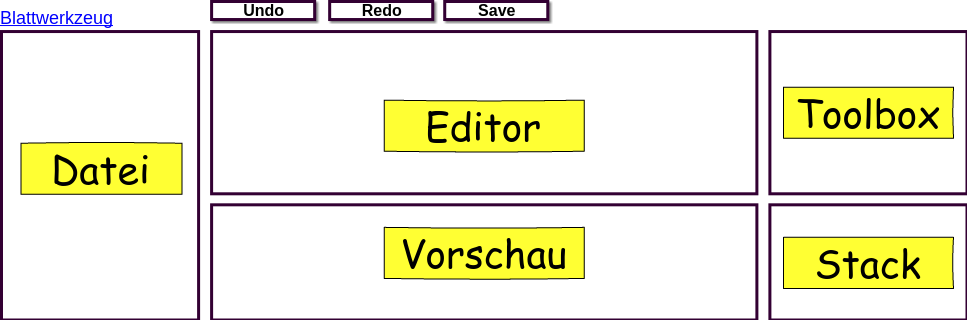
\includegraphics[width=\textwidth]{images/kap-4-editor-layout.png}
    \centering
    \caption{Layout des Editors}
    \label{pic:layout_editor}
\end{figure}
\end{description}

%%%%%%%%%%%%%%%%%%%%%%%%%%%%%%%%%%%%%%%%%%%%%%%%%%%%%%
\subsubsection{Bedienung}
\label{subsubsec04:editor_bedienung}

\begin{description}
\item[Einzelne Veränderungen] \hfill\\
Wie im Abschnitt~\ref{subsubsec04:editor_moegliche_aenderungen}, am Beispiel der Erstellung einer neuen Spalte fest zu stellen ist, sind Kombinationen von Veränderungen Auslöser für Fehler. So ist das Hinzufügen von neuen Spalten kein Problem, ungleich zum Hinzufügen einer neuen Spalte die ein \texttt{NOT NULL}-Constraint besitzt. \\
Des Weiteren ist bei einer Kette von Veränderung nicht immer feststellbar wie die Ursprungstabelle zu der Zieltabelle entwickelt wurde, wenn man die Zwischentabellen nicht kennt.
Zur genaueren Erläuterung betrachte man folgende Grafik:~\ref{pic:table_chain_changes_example}. 

\begin{figure}[ht]
    \frame{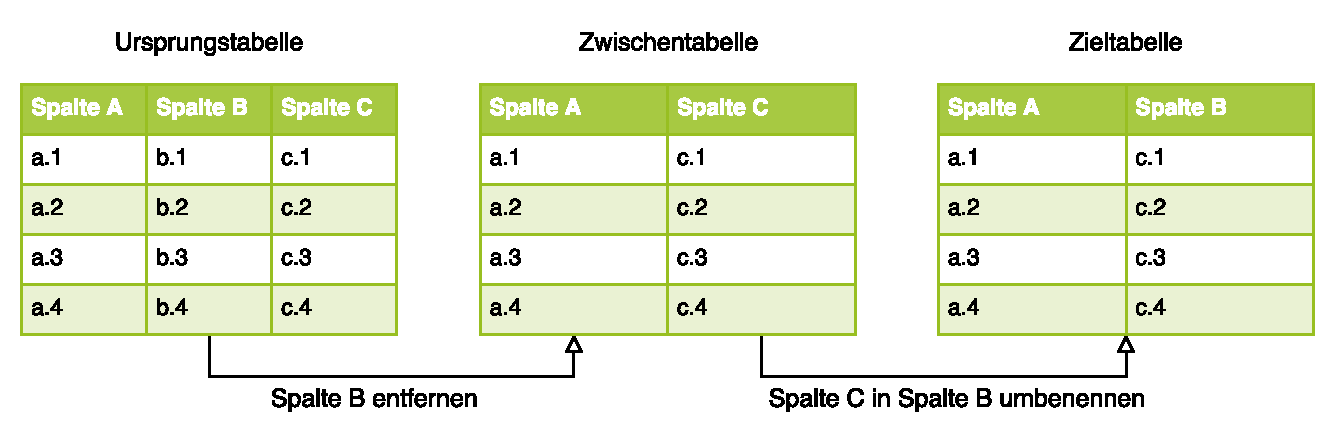
\includegraphics[width=\textwidth]{images/kap-4-chain-changes-ex.pdf}}
        \centering
        \caption{Exemplarische Veränderung einer Tabelle}
        \label{pic:table_chain_changes_example}
\end{figure}

Ohne Betrachtung der Werte und der Zwischentabelle, könnte davon ausgegangen werden, dass nur die Spalte C gelöscht wurde.
Aus diesen Gründen ist es sinnvoll, jeden Schritt im einzelnen zu betrachten und abzuspeichern, anstelle nur der Zieltabelle.
Zusätzlich bietet dies die Möglichkeit dem Benutzer genau mitzuteilen welche Veränderung fehlgeschlagen ist.


\item[Vorschau] \hfill\\
Der Editor zeigt nur die Informationen der Tabelle an. Zum leichteren Verständnis was die einzelnen Veränderungen bewirken, auf Hinsicht der Tabelle und der Daten, wurde eine Vorschau eingebaut. Die Vorschau zeigt die Tabelle in der typischen tabellarischen Darstellung an, mit ein paar Beispieldaten aus der Tabelle.\\
Eine solche Darstellung wurde schon in der Darstellung der Tabelleninhalte~\ref{subsubsec04:table_content} entwickelt. Diese wurde in einer eigenen Angular 2 Component geschrieben. Dadurch wurde die Wiederverwendbarkeit von Components benutzt, und wird direkt in die Componente des Editors eingebunden. Damit die Veränderung der Tabelle auch gleichzeitig in beiden Components sichtbar sind, wird das Objekt der Tabelle in einem Service gespeichert auf das beide Components zugreifen. In der Grafik~\ref{pic:angular2_architecture} wurde die allgemeine Architektur dargestellt.

Damit die Vorschau noch übersichtlicher wird, werden die einzelnen Spalten farblich gekennzeichnet:
\begin{itemize}
    \item Rot - Spalte wurde gelöscht
    \item Grün - Spalte wurde neu hinzugefügt
    \item Gelb - Spalte wurde verändert
\end{itemize}

\item[Undo \& Redo] \hfill\\
Typescript unterstützt unter anderem das Objekt Orientierte Paradigma, damit kann man auf bereits bekannte Entwurfsmuster der Objekt Orientierten Sprachen zurückgreifen. 
Um die ``Undo \& Redo'' Funktion einzubauen wird das Verhaltensmuster ``Command''\footnote{Kommando oder auch Befehl} verwendet.(Mehr dazu:~\ref{subsubsec04:cmd_pattern})

\item[Stack] \hfill\\
Beim Verwenden von ``Undo \& Redo'' und das dabei eingesetzte Entwurfsmuster Kommando sind die einzelnen Objekte in einer Liste abgelegt(siehe Kapitel:~\ref{subsubsec04:cmd_pattern}).
Durch die Erweiterung der einzelnen Klassen mit einer Funktion die eine String-Repräsentation des Objekts liefern, ist das Erstellen eines Stacks (siehe Grafik:~\ref{pic:stack}) möglich. Dieser zeigt die einzelnen Schritte an, welche bereits gemacht wurden. Mit einem Pfeil wird dargestellt an welcher Stelle im Stack man sich zurzeit befindet. Eine zusätzlich eingebaute Funktion ist, die Möglichkeit durch einen Klick an eine bestimmte Stelle im Stack zu springen. Dabei wird die Undo oder Redo Funktion mehrmals hintereinander ausgeführt, bis die Zielstelle im Stack erreicht ist. Wenn man sich nicht am Ende des Stacks befindet, werden alle Elemente vom Stackpointer bis zum Ende gelöscht, bevor ein neues Element hinzugefügt wird. 

\begin{figure}[ht]
    \frame{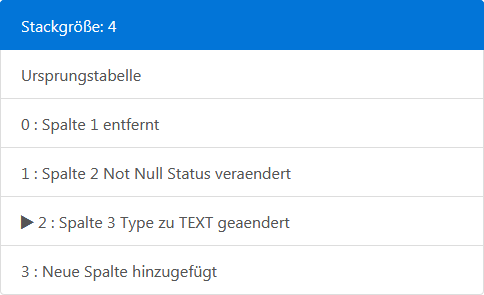
\includegraphics[width=0.7\textwidth]{images/kap-4-stack.png}}
        \centering
        \caption{Stack Beispiel}
        \label{pic:stack}
\end{figure}
\end{description}

Der Stack wird zusätzlich verwendet, um bei aufgetretenen Fehler darzustellen, welcher Schritt fehlgeschlagen ist. In diesem Fall wird der Eintrag im Stack, rot markiert.


%%%%%%%%%%%%%%%%%%%%%%%%%%%%%%%%%%%%%%%%%%%%%%%%%%%%%%
\subsubsection{Command Pattern}
\label{subsubsec04:cmd_pattern}

Während der Entwicklung einer Software sollte eine Architektur gut durchdacht sein. In der Objekt Orientierten Programmierung, in der wir uns in diesem Projekt bewegen, treten einige Probleme immer wieder auf. Für solche Probleme wurden in früheren Projekten bereits Lösungen entwickelt. Um ein ``Neuerfinden'' von bereits vorhandenen Lösungen zu vermeiden, wurde eine Reihe von Entwurfsmustern erstellt. \\
Eine Zusammenfassung an Entwurfsmuster für Softwareentwickler, wurde von der so genannten ``Gang of Four'' zusammengestellt und unter dem Namen ``Design Patterns: Elements of Reusable Object-Oriented Software'' veröffentlicht.

\begin{description}
\item[Allgemein] \hfill\\
Für die Veränderungen werden einzelne Funktionen benötigt, die ``Undo \& Redo'' Funktionen, im Zusammenhang mit dem Stack, dass zu jeder Funktion eine Funktion besteht, die diese Rückgängig macht. Dabei müssen die gegebenenfalls veränderten Zustände gespeichert werden, um diese wieder herzustellen. \\
Für solch eine Gegebenheit ist in dem Werk das Command\footnote{Befehl} im Buch genannt.
Zitat: 
\begin{quote}
``support undo. The Command's Execute operation can store state for reversing
its effects in the command itself. The Command interface must have an added
Unexecute operation that reverses the effects of a previous call to Execute.
Executed commands are stored in a history list. Unlimited-level undo and
redo is achieved by traversing this list backwards and forwards calling
Unexecute and Execute, respectively.'' ~\cite{Gamma1994}
\end{quote}

Das Command Pattern erlaubt es bestimmte Funktionen in ein Objekt zu kapseln. Diese können dann verwendet werden ohne die genaue Funktionalität des einzelnen Objektes kennen zu müssen.
Eine häufige Anwendungsmöglichkeit ist in der Implementierung von GUI-Elementen. Indem das Command ähnlich einer ``callback-function'' dient. Zusätzlich können die einzelnen Befehle in einer Liste gespeichert werden, um diese zu einem späteren Zeitpunkt auszuführen.
Die Struktur dieses Entwurfsmusters wird in folgender Grafik visualisiert:~\ref{pic:struct_cmd_gof}.

\begin{figure}[ht]
    \frame{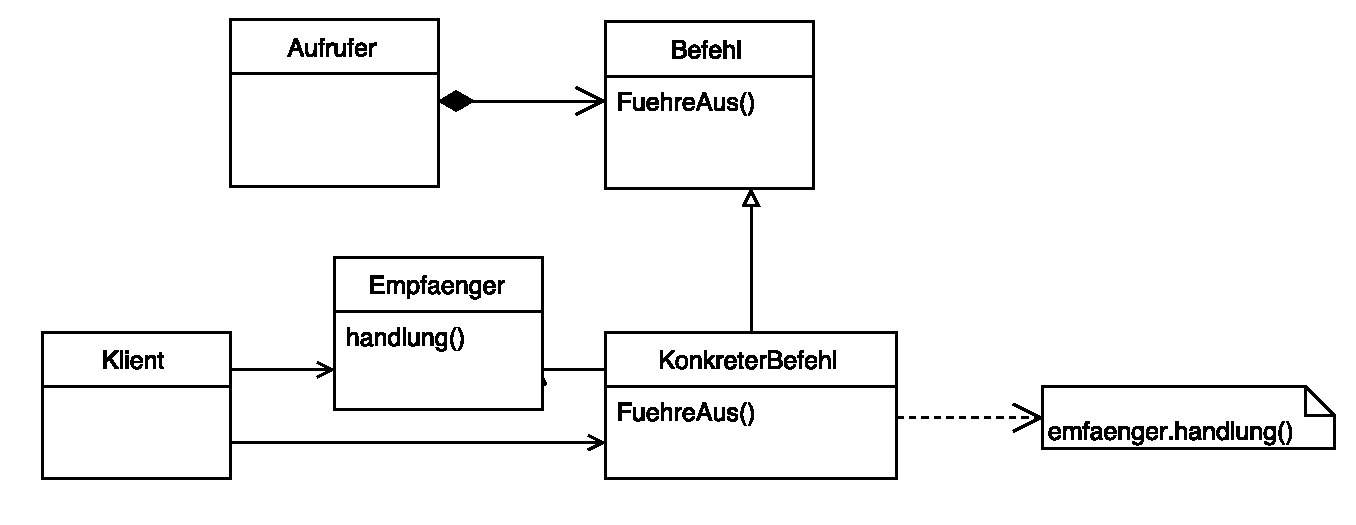
\includegraphics[width=\textwidth]{images/command_allg.pdf}}
        \centering
        \caption{Genreller Aufbau des Command}
        \label{pic:struct_cmd_gof}
\end{figure}

\item[Genereller Aufbau] \hfill\\
Anhand diesem Entwurfsmusters wurde für jede einzelne Veränderung an der Tabelle eine Klasse erstellt, die vom Typ Befehl ist. In jeder Klasse wurden die Funktionen zur Veränderung und deren Umkehrung implementiert. Zusätzlich speichert jede Klasse die nötigen Informationen und die alten Inhalte die verändert wurden. \\
In einer zusätzlichen Klasse, werden die einzelnen Befehle in einer Liste abgespeichert.
Für eine grafische Darstellung der Struktur siehe Grafik:~\ref{pic:struct_cmd_classes}
\begin{figure}[ht]
    \frame{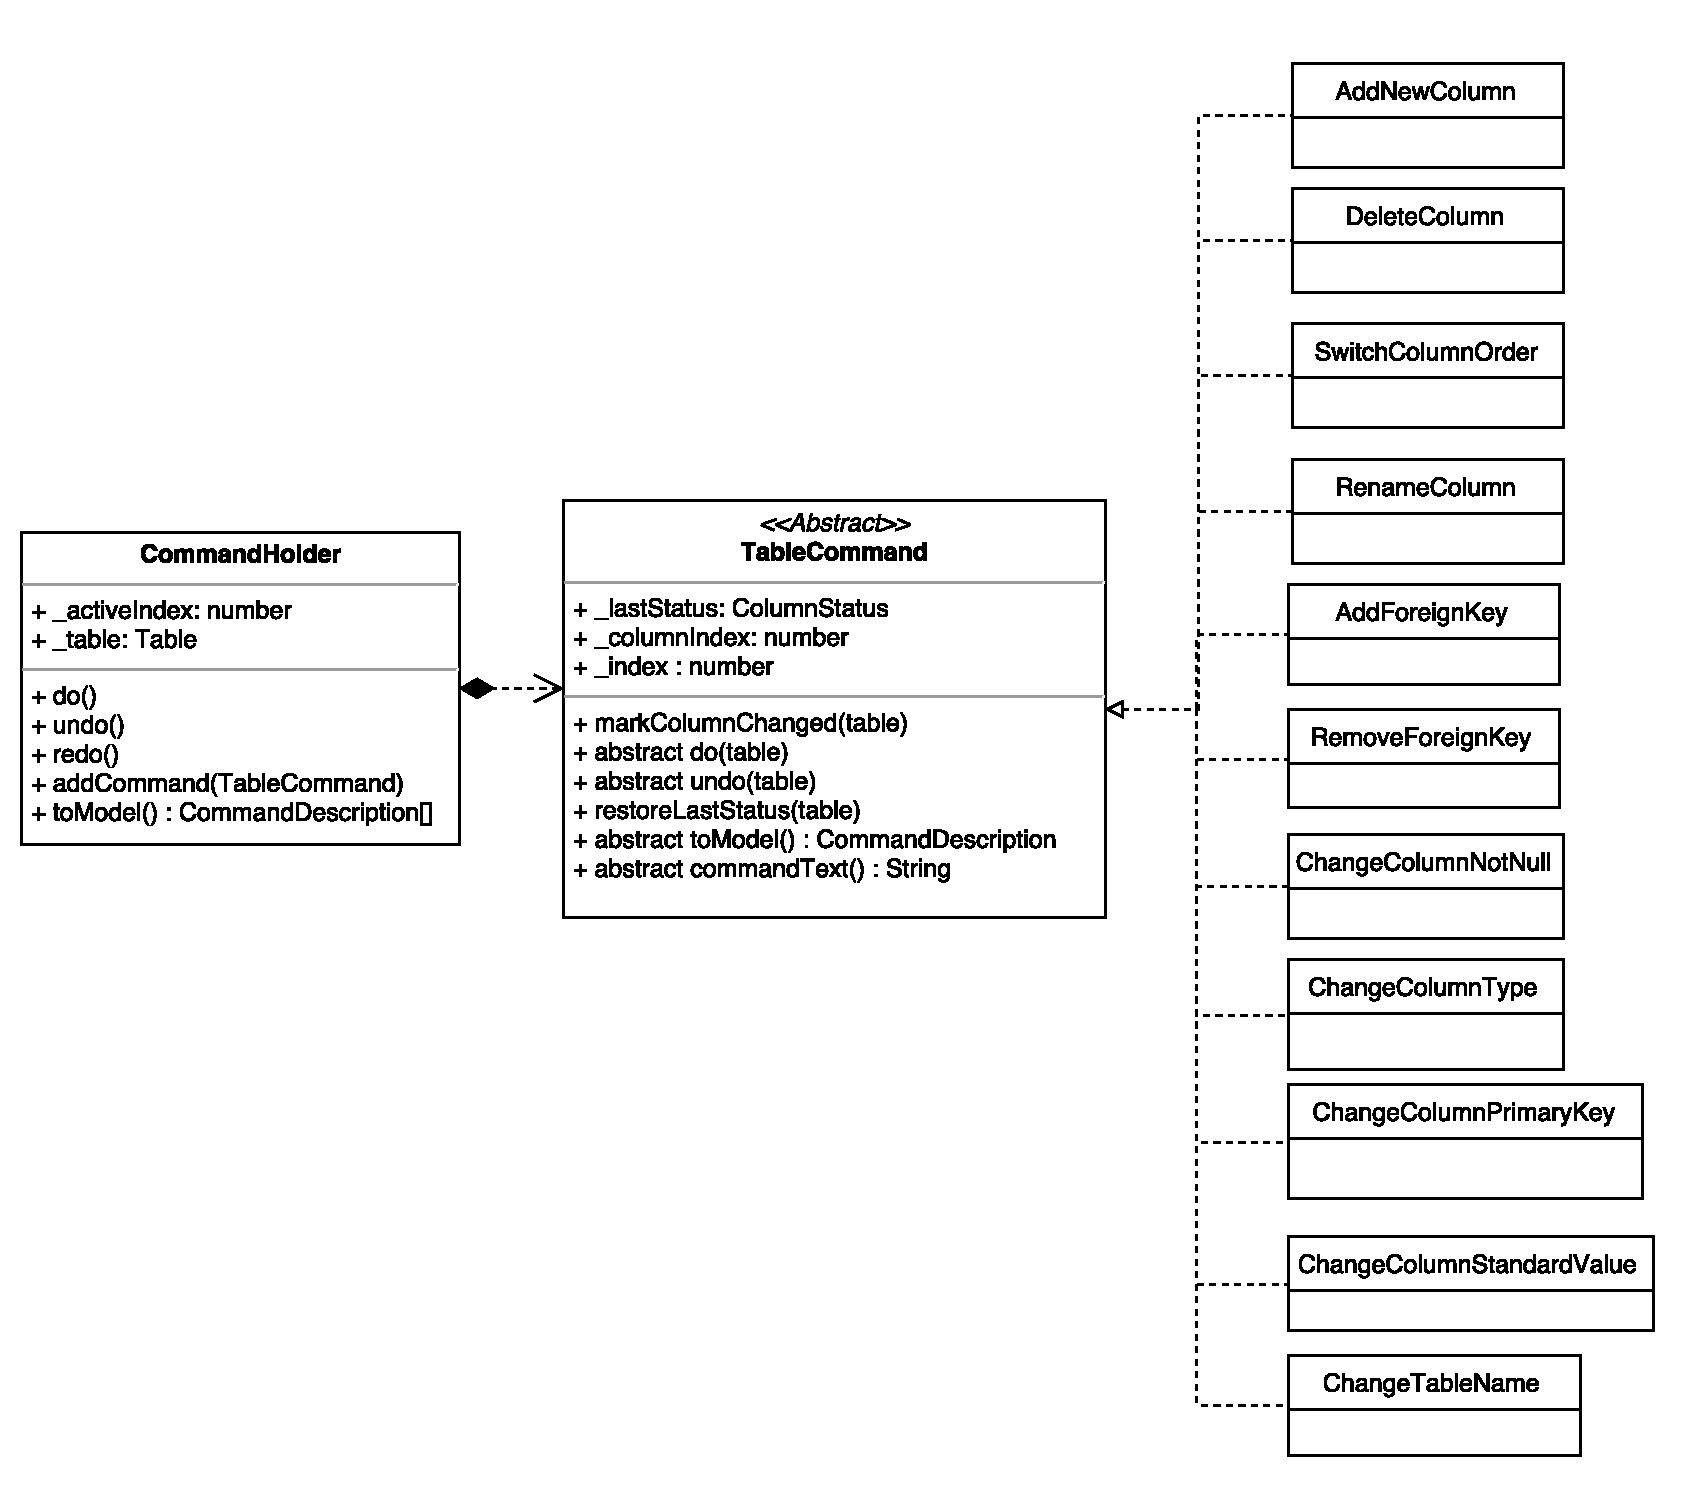
\includegraphics[width=\textwidth]{images/cmd_imple.pdf}}
        \centering
        \caption{Strukturaufbau der Klassen}
        \label{pic:struct_cmd_classes}
\end{figure}

\item[Konvertierung Interfaces] \hfill\\
Jede Befehlsklasse besitzt eine Funktion zur Erstellung einer \texttt{JSON}-Repräsentation von sich selbst. Diese kann direkt an den Server versendet werden, um die Änderungen in der Datenbank durchzuführen.

\item[Textuelle Darstellung] \hfill\\
Zusätzlich kann jede einzelne Klasse eine textuelle Darstellung ausgeben, um diese auf dem Stack anzeigen zu können.
\end{description}

%%%%%%%%%%%%%%%%%%%%%%%%%%%%%%%%%%%%%%%%%%%%%%%%%%%%%%
\subsubsection{Kommunikation mit dem Server}
\label{subsubsec04:kommunikation_cs}
In diesem Abschnitt wird die Kommunikation beschrieben. Wie der Client Anfragen an den Server verschickt und welche Antwort erwartet wird.
Die Serverseitige Kommunikation wird im Kapitel:~\ref{subsubsec04:sinatra_client_reaction} beschrieben.

Für alle Anfragen braucht der Server einen Identifikator, der das Projekt definiert und den Namen der Datenbank. Die Anfragen werden per \texttt{HTTP}-Befehle an den Server geleitet.\footnote{Genaueres siehe: \url{https://marcusriemer.de/static/marcus-riemer-thesis-blattwerkzeug.pdf}}

\begin{description}
\item[Tabelleninhalte vom Server beantragen] \hfill\\
Für die Anfrage der Daten einer Tabelle wird der Tabellenname benötigt. Hinzu kommt, dass in der Ansicht der Daten, durch das Pagination (siehe Kapitel:~\ref{subsubsec04:anz_schema}), dem Server mitgeteilt werden muss, wie viele und ab welchen Tabelleneintrag die Daten erwartet werden.

Als Antwort ist ein 2-Dimensionales Array zu erwarten, welches die Spalten und all deren Zeilen enthält.

\item[Neue Tabellen erstellen] \hfill\\
Für das Erstellen neuer Tabellen muss in dem \texttt{Body} des \texttt{HTTP}-Befehls ein \texttt{JSON}-Objekt sich befinden, welches die zu erstellende Tabelle mit allen Informationen repräsentiert.

Als Antwort erhält der Client das neue komplette Schema zurückgeschickt. Damit kann der Client das Schema aktualisieren.
Dies erhöht den Datentransfer zwischen Server und Client. Eine andere Möglichkeit wäre, das Schema des Clients mit dem vorhandenen Objekt separat zu erweitern. Dies verringert den Datentransfer, kann aber bei Kommunikationsfehlern zu nicht synchronisierten Zuständen führen. Um dem gegen zu wirken, wird der Zustand des Servers als richtig angenommen und an den Client verschickt.

\item[Tabellen löschen] \hfill\\
In diesen Fall wird nur der Name der Tabelle verschickt. 

Die Antwort ist wieder das komplette aktualisierte Schema.

\item[Tabellen verändern] \hfill\\
In dem \texttt{Body} der Anfrage, ist eine Liste an einzelnen Befehlen~\ref{subsubsec04:cmd_pattern} die an einer Tabelle ausgeführt werden sollen.

Die Antwort, sollten keine Probleme auftreten, ist das aktualisierte Schema.

\item[Fehler beim Ausführen der Befehle] \hfill\\
Beim Erstellen, Löschen und Verändern wird die von der Datenbank mitgeteilte Fehlernachricht an den Client versendet.
Dies können Fehler sein, wie das Erstellen einer Tabelle mit einem Bereits vergebenen Namen oder auch Konsistenzverstöße des Schemas.

Beim Editieren einer Tabelle, wird zusätzlich der genaue Schritt mitgeteilt an welchem ein Fehler aufgetreten ist. Dies wird, wie im Abschnitt~\ref{subsubsec04:editor_bedienung} verwendet, um den Fehler im Stack darzustellen.
\end{description}


%%%%%%%%%%%%%%%%%%%%%%%%%%%%%%%%%%%%%%%%%%%%%%%%%%%%%%
\subsubsection{Problematiken}
\label{subsubsec04:problematik}

Während der Entwicklung des Clients kamen einige Probleme auf, die auf mehrere Weisen gelöst werden konnten. In diesem Abschnitt soll besprochen werden, welche Probleme aufkamen mit den möglichen Lösungen und einer Begründung warum die jeweilige Lösung gewählt wurde.

\begin{description}
\item[Multiple Tabellen simultan verändern] \hfill\\
Jede Veränderung einer Tabelle wird erst übernommen, wenn ein Speicher-Button gedrückt wird. Damit kam die Frage auf, wie damit umgegangen werden soll, wenn man während der Bearbeitung einer Tabelle, denn Editiervorgang verlässt und eine andere Tabelle bearbeitet.
Damit wäre es möglich zwei Tabellen simultan zu verändern. \\
Dies bietet eine Vielzahl an möglichen Problemen, die nur schwer vorhersehbar sind. Zusätzlich wäre eine sehr klare und detaillierte Kommunikation notwendig bei der Benutzung der Software. Sollte ein Benutzer eine Änderung an einer Tabelle gemacht haben und den Editorvorgang verlassen haben, muss zu jedem Zeitpunkt folgendes klar definiert sein. Hat der Benutzer den Editiervorgang verlassen, um eine andere Änderung durchzuführen, oder weil er den Vorgang abbrechen will. In Anbetracht der unvorhersehbaren Probleme, ist der Gewinn einer solchen Funktionalität recht gering. Zusätzlich sollte Einsteigern im Thema Datenbanken verständlich gemacht werden, dass die Migration von Datenbanken sich immer nur auf das Nötigste beziehen sollte, mit so wenig und kleinen Veränderungen wie möglich. Gerade bei den ersten Projekten, die keinen großen Umfang aufweisen, sollte eine Migration durch gute Vorausplanung verhindert werden. \\
Somit ist es nicht möglich mehrere Tabellen gleichzeitig zu verändern. Da aber während einer Veränderung, der Wunsch bestehen könnte, sich die anderen Tabellen anzusehen ohne das der Stack\footnote{die bereits durchgeführt, aber noch nicht gespeicherten Veränderungen} gelöscht wird, besteht die Möglichkeit den Editiermodus zu verlassen, dass Schema zu betrachten und den Editiervorgang fortzusetzen. Beim Betreten eines Editiermodus einer anderen Tabelle, wird der Benutzer darauf aufmerksam gemacht, dass das Betreten eines anderen Editiervorgangs, den bereits vorhandenen Stack löscht.

\item[Undo vs. selbst verändern] \hfill\\
Die Undo \& Redo Funktion (siehe Kapitel:~\ref{subsubsec04:editor_bedienung}) wurde eingebaut,als Erleichterung für den Nutzer, um eine falsche Aktion wieder Rückgängig zu machen. Der durch die Undo \& Redo Funktion entstandene Stack wird auch genutzt, um diesen zum Server zu schicken. \\
Neben der Benutzung von Undo ist es auch möglich die Änderung selbst Rückgängig zu machen. Als Beispiel wäre das Hinzufügen eines \texttt{NOT NULL} Constraints, und dieses wieder manuell zu entnehmen, im Gegensatz zur Benutzung der Undo-Funktion. 
Dies würde zu zwei verschiedenen Stacks führen, die auch anders auf Serverseite durchgeführt werden würden. (Siehe Grafik:~\ref{fig:self_vs_undo})

\begin{figure}[ht]
  \begin{subfigure}[b]{0.45\textwidth}
    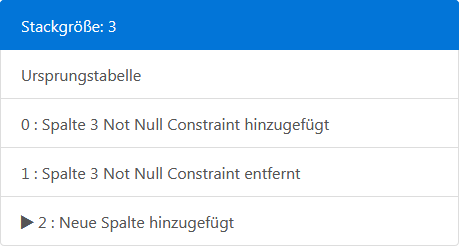
\includegraphics[width=\textwidth]{images/kap-4-self_stack_change.png}
    \caption{Manuell Rückgängig}
    \label{fig:stack_self}
  \end{subfigure}\hfill
  \begin{subfigure}[b]{0.45\textwidth}
    \includegraphics[width=\textwidth]{images/kap-4-undo_stack_change.png}
    \caption{Nutzung von Undo}
    \label{fig:stack_undo}
  \end{subfigure}
  \caption{Vergleich manuell Rückgängig vs. Undo}
  \label{fig:self_vs_undo}
\end{figure}

Dadurch könnten Fehler auftreten, wenn Änderungen auf dem Server durchgeführt werden, von denen der Benutzer ausging sie wurden Rückgängig gemacht. Eine mögliche Lösung des Problems ist die ``Stack Optimierung'' die im nächsten Abschnitt besprochen wird und aus welchem Grund diese nicht von Vorteil ist. \\
Bei einigen Änderungen kann man die Absicht des Benutzers nicht abschätzen, und verhindert gegebenenfalls Änderungen die vom Benutzer gewollt sind. Mit der Anzeige des Stacks wird dem Benutzer angezeigt, welche Schritte durchgeführt werden.
Dies ist ein mögliches Thema, welches in weiterer Entwicklung der Software beachtet werden könnte. Mögliche Lösungen können sich ergeben nach Absprache mit Benutzern. 

\item[Stack Optimierung] \hfill\\
Stack Optimierung ist die Verallgemeinerung des Problems ``Undo vs. selbst verändern''. Es gibt viele Ketten an Veränderungen die zusammengefügt oder optimiert werden könnten. Einige Beispiele wären:
\begin{itemize}
    \item Verändern einer Spalte die danach gelöscht wird
    \item Manuelles rückgängig machen von Veränderungen
    \item Eine Spalte mehrmals Umbenennen
\end{itemize}

Die jeweiligen Lösungen dafür wären:
\begin{itemize}
    \item Veränderungen nicht durchführen, Spalte sofort löschen
    \item Änderung gar nicht erst durchführen
    \item Spalte direkt auf den letzten Namen ändern
\end{itemize}

Alle diese Änderungen könnten aber von dem Benutzer genau in dieser Weise gewollt sein. So könnte ein mehrfaches Umbenennen einer Spalte die Folge sein, wenn bei zwei Spalten die Namen vertauscht werden sollen und dafür der Spaltenname einer Spalte einen temporären Namen erhielt. \\
Sollte eine Optimierung des Stacks dynamisch schon während der Bearbeitung der Tabelle stattfinden, könnte dies zur Verwirrung des Benutzers führen, wenn einzelne Schritte aus dem Stack verschwinden und dann auch nicht mehr per Undo erreicht werden können.
Wenn die Optimierung nach dem Speichern angewendet wird, ist die Benachrichtigung während welchen Schrittes ein Fehler aufkam deutlich erschwert. \\
Die letzten beiden Punkte sind in Anbetracht des ersten Punktes, der Vorhersage was vom Benutzer wirklich gewollt ist, einfacher zu Lösen und weisen trotzdem einen hohen Aufwandswert auf, für den dafür gewonnen Nutzen. \\
Dieses Thema ist eine Optimierung die zu keiner besseren Benutzung der Software selbst führt und der Optimierungsgrad ist relativ gering im Vergleich zum Arbeitsaufwand, und wurde aus diesen Gründen in dieser Arbeit nicht weiter bearbeitet. In der weiteren Entwicklung der Software, kann dieses Thema ein Ansatzpunkt sein. 
\end{description}




\newpage
\subsection{Server}
\label{subsec04:server}
Im folgendem Kapitel, wird die Implementierung des Servers beschrieben. Der Aufbau von Blattwerkzeug besitzt eine starke Trennung zwischen Client und Server. Dies ermöglichte es, diese beiden Gebiete von einander getrennt zu implementieren. Die bereits vorhandene Testmöglichkeit des Server, erlaubt es alle Funktionalitäten zu testen, ohne die Verwendung eines Clients. \\
Der Server bietet eine direkte Schnittstelle für die Kommunikation mit der Datenbank, welche erlaubt die eigentlichen Aktionen auszuführen.

\subsubsection{Sinatra reagieren auf Anfragen}
\label{subsubsec04:sinatra_client_reaction}
In Sinatra werden die Anfragen durch ein \texttt{REST}-artigem System angesprochen.
Für die jeweiligen Anfragen wurden URLs bestimmt, mit denen die einzelnen Funktionen von Clients angesteuert werden konnten.
Die möglichen Anfragen an den Server sind:
\begin{itemize}
    \item Einen Satz von Daten einer Tabelle
    \item Die Anzahl von vorhandenen Daten in einer Tabelle
    \item Löschen einer Tabelle
    \item Anlegen einer neuen Tabelle
    \item Editieren einer Tabelle
\end{itemize}

Dabei wurde zur Vorbeugung von ``SQL-Injections''\footnote{\url{https://de.wikipedia.org/wiki/SQL-Injection}} darauf geachtet durch Prüfung, ob eine Tabelle zu der Informationen oder Änderungen angefragt wurden, auch wirklich besteht.

\subsubsection{Foreign Keys der Tabellen}
\label{subsubsec04:fk_table_server}
Das Schema wurde bereits an den Client versendet. Um die Foreign Keys dem Schema anzuhängen, wurde zuerst die Struktur der Foreign Keys bestimmt. \\
Die Informationen von Foreign Keys einer Tabelle kann man mit der Verwendung von \texttt{PRAGMAS} erhalten.
\texttt{PRAGMA}-Statement ist eine Erweiterung in SQLite, diese wird für die modifizierung der SQLite Operationen und zum erhalt von internen (nicht Tabellen) Informationen genutzt.\cite{sqlite_pragma} \\

Die Ausgabe des \texttt{PRAGMA} ``foreign\_key\_list''\footnote{\url{https://sqlite.org/pragma.html\#pragma_foreign_key_list}} enthält die nötigen Informationen. Sie bietet eine Liste einer Liste von zusammengesetzten Foreign Keys. Diese werden unter anderem durch drei Eigenschaften dargestellt:
\begin{itemize}
    \item den Spaltennamen der Tabelle die ein Foreign Keys Constraint besitzt
    \item auf welche Tabelle dieser Foreign Keys verweist
    \item zu welcher Spalte dieser Tabelle genau verwiesen wird
\end{itemize}

Foreign Keys auf Spaltenebene zu speichern erschien somit nicht sinnvoll. Wegen der Ausgabe des \texttt{PRAGMA} und das Foreign Keys aus mehreren Foreign Keys zusammengesetzt sein können, werden die Informationen zu Foreign Keys auf Tabellenebene gespeichert. \\
Diese werden mit Anlehnung an die Ausgabe des \texttt{PRAGMA} gespeichert. Es wird eine Liste einer Liste zusammengesetzter Foreign Keys gespeichert, die die drei Information direkt aus dem \texttt{PRAGMA} speichert. \\
Dies wird dann zusammen mit dem bereits versendeten Schema an den Client geliefert.   

\subsubsection{Typsicherung der Tabellenspalten}
\label{subsubsec04:typsicherung}
Die dynamische Typisierung von Spalten ist in SQLite eine Ausnahme verglichen mit anderen Datenbanken, wie schon im Kapitel:~\ref{subsubsec03:zu_entwickeln-Datentypen} erwähnt wurde. \\
Aus diesem Grund ist dafür gesorgt, dass die Typen in Blattwerkzeug sich ähnlicher zum Standard vom SQL verhalten. Dafür werden die Werte die in eine Tabelle eingetragen werden je nach Typ überprüft.
SQLite besitzt drei Möglichkeiten Werte nach einem bestimmten Muster zu prüfen. \\
Der \texttt{LIKE}-Operator bietet zwei Wildcards im zu vergleichenden Muster:
\begin{itemize}
    \item ``\_'' ein beliebiges Zeichen
    \item ``\%'' eine beliebige Anzahl an Zeichen
\end{itemize}
In Abfragen ist der \texttt{LIKE}-Operator häufig zu gebrauchen und nützlich.

Der \texttt{GLOB}-Operator ist sehr ähnlich zu dem \texttt{LIKE}-Operator, er ist zusätzlich Case-Sensitive und bietet Wildcards mit gleicher Funktionalität wie der \texttt{LIKE}-Operator und einer Möglichkeit ein Zeichen variabel aus einer Menge zu setzen. \\
Die Funktionalität vom \texttt{GLOB}-Operator und \texttt{LIKE}-Operator sind nicht ausreichend für die Überprüfung eines Wertes, ob dieser die Kriterien eines Typs erfüllt.

SQLite besitzt zusätzlich einen ``REGEXP''-Operator der prüfen kann, ob ein String\footnote{Zeichenkette} einem Regulären Ausdruck entspricht.
Der ``REGEXP''-Operator ist in SQLite nativ nicht implementiert, um die SQLite Datenbankbibliothek so klein wie möglich zu halten. Somit muss zur Laufzeit eine solche Funktion implementiert und hinzugefügt werden. \\
Die Schnittstelle von Ruby, in dem der Server geschrieben wurde, besitzt eine ``create\_\-function''-Funktion, um bei der Verbindung mit einer SQLite Datenbank, eine Funktion zu definieren, die dann verwendet werden kann. Damit wurde eine Funktion definiert für den ``REGEXP''-Operator. Der Quelltext dieser Funktion ist in Listing~\ref{lst:regexp_impl} dargestellt.

\lstinputlisting[
  language=ruby,
  caption=Implmentierung einer Funktion für den ``REGEXP''-Operator,
  label=lst:regexp_impl,
  float=h,
  numbers=left
]{snippets/regexp_impl.rb} 

Die Funktion überprüft im ersten Schritt, ob der übergebene Wert ein leerer String ist. Dies verhindert, dass \texttt{REGEXP} einen Fehler auslöst, da ein leerer String mit dem übergebenen Muster nicht übereinstimmt. Die Datenbank hat bereits mit dem \texttt{NOT NULL}-Constraint eine Überprüfung, ob ein Wert \texttt{NULL} sein darf oder nicht. Aus diesem Grund werden leere Strings nicht von der Funktion überprüft. \\
Der Rest der Funktion benutzt die Ruby Implementierung einer \texttt{REGEXP}-Funktion.\footnote{\url{https://ruby-doc.org/core-2.1.1/Regexp.html}}
Nachdem der ``REGEXP''-Operator verwendet werden kann, wird bei der Definition einer Spalte die Möglichkeit geboten, ein \texttt{Contraint}\footnote{\url{https://sqlite.org/lang_createtable.html}} zu definieren.
Für jeden der vorgesehenen Typen wurde ein \texttt{Contraint} erstellt, mit einer individuellen Fehlermeldung. Die vier Typen sind:
\begin{itemize}
    \item \texttt{TEXT} - Eine Menge an beliebigen Zeichen, dafür ist ein Constraint nicht nötig
    \item \texttt{BOOLEAN} - Der Wert darf nur von Wert von 1 oder 0 annehmen, dies kann mit Vergleichsoperatoren implementiert werden (siehe:~\ref{lst:regex_bool})
    \item \texttt{INTEGER} - Eine Vorzeichen gebundene ganze Zahl, dafür wird der ``REGEXP''-Operator verwendet, um sicher zustellen, dass nur Zahlen in dem Wert enthalten sind (siehe:~\ref{lst:regex_integer})
    \item \texttt{FLOAT} - Eine Vorzeichen gebundene reelle Zahl, dafür wird der ``REGEXP''-Operator verwendet, damit auch nur solche Zahlen angenommen werden (siehe:~\ref{lst:regex_float})
    \item \texttt{URL} - Ein zusätzlicher Typ, der in standard Datenbanken nicht vorhanden ist, soll aber für die junge Zielgruppe ein weiterer Zusatz sein, der die Möglichkeit bietet URLs in einer Datenbank zu speichern. (siehe:~\ref{lst:regex_url})
\end{itemize}

\lstinputlisting[
  language=sql,
  caption=Implementierung des \texttt{BOOLEAN}-Constraint,
  label=lst:regex_bool,
  float=p,
  numbers=left
]{snippets/regex_bool.sql}

\lstinputlisting[
  language=sql,
  caption=Implementierung des \texttt{INTEGER}-Constraint,
  label=lst:regex_integer,
  float=p,
  numbers=left
]{snippets/regex_integer.sql}

\lstinputlisting[
  language=sql,
  caption=Implementierung des \texttt{FLOAT}-Constraint,
  label=lst:regex_float,
  float=p,
  numbers=left
]{snippets/regex_float.sql}

\lstinputlisting[
  language=sql,
  caption=Implementierung des \texttt{URL}-Constraint,
  label=lst:regex_url,
  float=p,
  numbers=left
]{snippets/regex_url.sql}
  

\subsubsection{Anfragen - Darstellung}
\label{subsubsec04:anfragen_darstellung}

Wie schon im Kapitel~\ref{subsubsec04:anz_schema} wurde das Schema bereits an den Client versendet, mit der Erweiterung der Foreign Keys. (siehe Kapitel:~\ref{subsubsec04:fk_table_server}) \\
Für die Darstellung der einzelnen Tabelleninhalte, mit der Möglichkeit der Pagination~\ref{subsubsec04:table_content}, soll nur eine gewisse Anzahl an Daten aus einer Tabelle an den Client gesendet werden.

Die erste Möglichkeit nur eine bestimmte Anzahl an Daten an den Client zu schicken, wäre alle Daten von der Datenbank auf dem Server zu filtern und diese an den Client zu schicken. Dabei wäre das Problem, dass bei einer Tabelle mit vielen Inhalten viel Datentransfer statt finden würde. \\
Um den Datentransfer so niedrig wie möglich zu halten, werden die ``\texttt{LIMIT}''- und ``\texttt{OFFSET}''-Funktionen benutzt. 

Mit der ``\texttt{LIMIT}''-Funktion kann genau angegeben werden wie viele Daten aus der Tabelle wiedergegeben werden. Somit kann die Anzahl an Daten aus der Datenbank erfragt werden, die pro Page angezeigt werden sollen.

Mit der ``\texttt{OFFSET}''-Funktion, wird eine Anzahl an Daten übersprungen bei der Ausgabe. Somit werden bei einem \texttt{OFFSET 10} erst die Daten ab dem 11 Eintrag wiedergegeben. 

Zusätzlich zu den anzuzeigenden Daten auf dem Client, ist für die Pagination die Anzahl an vorhandenen Daten in der Tabelle nötig. Dafür wurde der ``\texttt{COUNT}''-Operator verwendet. Dieser wird in der Form ``\texttt{SELECT COUNT(*) FROM ...}'' verwendet. Dabei steht das ``\texttt{*}'' für alle Einträge, wobei das ``\texttt{COUNT}'' die Anzahl dieser zurückliefert.  

\subsubsection{Anfragen - Entfernen/Hinzufügen}
\label{subsubsec04:anfragen_editor_add_remove}

\begin{description}
\item[Tabellen entfernen] \hfill\\
Beim Entfernen einer Tabelle wurde keine weitere Funktionalität benötigt als die schon erwähnte Prüfung, ob die besagte Tabelle vorhanden ist. (siehe Kapitel:~\ref{subsubsec04:sinatra_client_reaction})\\
Die SQL-Datenbank meldet einen Fehler bei existenz eines Foreign Keys, der auf die zu löschende Tabelle, verweist. Der Fehler wird, an den Benutzer weitergeleitet. 

\item[Tabellen hinzufügen] \hfill\\
Bei der Anfrage zum Erstellen einer Tabelle erhält der Server im \texttt{Body} der Anfrage eine \texttt{JSON} Repräsentation der Tabelle. \\
Diese ist äquivalent zu der \texttt{JSON} Darstellung die bereits Verwendet wurde, um die einzelnen Tabellen vom Server an den Client zu senden. Damit wird die bereits implementierte Tabellen-Klasse verwendet, um das \texttt{JSON}-Objekt in ein Ruby Objekt zu konvertieren, für die weitere Verwendung. \\
Das Objekt einer Tabelle muss zu einem SQL-CREATE\_TABLE-Statement umgeformt werden, um dieses dann an die Datenbank zu senden. Die möglichen Fehler werden von der Datenbank geprüft und gegebenenfalls an den Client weiter gesendet. Einige typische Fehler, wie die Einzigartigkeit des Tabellennamens könnten bereits auf Clientsseite geprüft werden. Dies ist bei weiteren Optimierungen in Betracht zu ziehen. Die vorhandene Implementierung ermöglicht es solche Optimierung in der Zukunft einzubauen. Durch eine große Menge möglich auftretender Fehler und um eine Vermischung von Client- und Datenbankseitiger Fehlererkennung zu verhindern, wurde die ganze Fehlererkennung an die Datenbank ausgelagert.
\end{description}

\subsubsection{SQLite vs. Ruby-Migration}
\label{subsubsec04:sql_vs_ruby}
Für die Kommunikation mit der Datenbank gibt es die Möglichkeit der Verwendung von SQL oder der in Ruby integrierten ``Migration''.
Die Ruby Migration bietet die Möglichkeit Datenbanken zu verändern, dabei neue Tabellen erstellen, Tabellen zu verändern oder Tabellen zu löschen. Die Migration ist dabei Datenbanken unabhängig, somit wäre der Wechsel von SQLite zu einem anderen Datenbanksystem vereinfacht. In Hinblick auf die zur Verfügung gestellten Veränderungen (siehe Kapitel:~\ref{subsubsec04:editor_moegliche_aenderungen}), und der Typsicherung~\ref{subsubsec04:typsicherung} wurde sich für die Implementierung mit SQL-Statements entschieden. \\
Eine Veränderung des Tabellennamens und das Hinzufügen neuer Spalten oder kompletten Tabellen ist in SQLite und Ruby Migration möglich. Für eine Kategorisierung welche Veränderungen durch welche Schnittstellen nativ möglich sind siehe Tabelle:~\ref{tbl:sql_vs_ruby}

\begin{table}[]
\centering
\begin{tabular}{l|ll}
\hline
\multicolumn{1}{c}{\textbf{Veränderung}}           & \multicolumn{1}{c}{\textbf{SQLite}} & \multicolumn{1}{c}{\textbf{Ruby Migration}} \\ \hline
Reihenfolge vertauschen        &          &                         \\ \hline
Primary Key setzen/entfernen   &          &                         \\ \hline
Spaltentypen verändern         &          &                         \\ \hline
Check Constraint setzen        & \multicolumn{1}{c}{$\surd$}(im Create Table)         &                         \\ \hline
Not Null setzen/entfernen      &          &                         \\ \hline
Default Value setzen/entfernen &                 &  \multicolumn{1}{c}{$\surd$}                \\ \hline
Spalte entfernen               &                 &  \multicolumn{1}{c}{$\surd$}                \\ \hline
Foreign Keys setzen/entfernen  &                 &  \multicolumn{1}{c}{$\surd$}                \\ \hline
Tabellen Namen verändern       & \multicolumn{1}{c}{$\surd$}         &  \multicolumn{1}{c}{$\surd$}                \\ \hline
Spalte Hinzufügen              & \multicolumn{1}{c}{$\surd$}         &  \multicolumn{1}{c}{$\surd$}                \\ \hline
\end{tabular}
\caption{Native Funktionen in SQLite \& Ruby Migration}
\label{tbl:sql_vs_ruby}
\end{table}

Die Typsicherung ist ein wichtiger Aspekt in dieser Software (siehe:~\ref{subsubsec04:typsicherung}), dies ist von Ruby Migration nicht direkt unterstützt und müsste per zusätzliches SQL-Statement erreicht werden, ähnlich wie die Veränderung der Spaltenreihenfolge. \\
Es müssten somit für die Ruby Migration Sonderfälle integriert werden, um jede Veränderung abzubilden. \\
SQLite besitzt nativ nur die Möglichkeit Tabellennamen zu ändern und das Hinzufügen einer neuen Spalte. Jedoch bieten die SQLite Entwickler einen allgemeingültigen Algorithmus an, mit dem sich alle möglichen Veränderungen realisieren lassen:\cite{sqlite_doc_alter}

\begin{enumerate}\label{enum:sql_algo}
    \item Wenn Foreign Keys aktiviert sind, müssen diese deaktiviert werden
    \item Starten einer Transaktion
    \item Alle Indizes und Trigger speichern, die mit dieser Tabelle verbunden sind
    \item Eine neue Tabelle erstellen, die das gewünschte Format besitzt. Benenne diese mit einem temporären Namen
    \item Übermittle alle Inhalte der alten Tabelle in die neue Tabelle
    \item Lösche die alte Tabelle
    \item Verändere den Namen der neuen Tabelle in den gewünschten Namen
    \item Erstelle Indizes und Trigger nach dem Vorbild der alten Tabelle
    \item Lösche alle Views die durch die Veränderung betroffen sind und rekonstruiere diese
    \item Sollten Foreign Keys ursprünglich aktiviert sein, prüfe die Konsistenz der Datenbank durch ``PRAGMA foreign\_key\_check''
    \item Commit die Transaktion
    \item Aktiviere die zuvor deaktivierten Foreign Keys
\end{enumerate}

Da dieser Algorithmus bereits allgemeingültig ist und dieser für Veränderungen implementiert werden müsste, die durch Ruby Migration nicht realisiert werden können, wurde der SQLite Algorithmus für alle Veränderungen verwendet. Zusätzlich müssen keine ``Mischlösungen'' implementiert und weitere Ruby Bibliotheken eingebunden werden.    

\subsubsection{Anfragen - Editieren}
\label{subsubsec04:anfragen_editor_edit}
In diesem Abschnitt wird die Implementierung erläutert, wie einzelne Tabellen auf der Serverseite und somit in der Datenbank selbst verändert werden. Dabei wird der von SQLite vorgegebene Algorithmus zur eigentlichen Migration verwendet(siehe:~\ref{subsubsec04:sql_vs_ruby}).

Die Daten die vom Client bei einer Anfrage zum Verändern einer Tabelle versendet werden, sind in einer Liste bestehend aus JSON-Objekten, die die einzelnen Veränderungen darstellen. (genaueres siehe:~\ref{subsubsec04:kommunikation_cs})
Auf dem Server wird der gleiche Vorgang realisiert, der auf dem Client bereits realisiert wurde. Die einzelnen Befehle des Command Patterns, werden auf dem Server durch einzelne Funktionen abgebildet. Die zu jedem Command, auf Clientsseite, vorhandene ``Undo''-Funktion ist auf dem Server nicht abgebildet. Zu dem Zeitpunkt, wenn eine Änderung auf dem Server durchgeführt werden soll, sind die einzelnen Veränderungen bereits fest, und müssen nicht rückgängig gemacht werden.
Hierbei werden bereits vorhandene Funktionen verwendet. Es wird ein Objekt aus der Tabelle, die Verändert wird, von der Datenbank erstellt. Die Funktion Objekte aus Tabellen der Datenbank zu erschaffen, wurde bereits von Marcus Riemer erstellt. Die erstellten Funktionen in Anlehnung an die Commands vom Client, verändern das Objekt. Nachdem das Objekt verändert wurde, kann dieses auf die gleiche Weise wie beim Erstellen einer neuen Tabelle zu einem SQL-CREATE\_TABLE-Statement konvertiert werden.

\begin{description}
\item[Zuweisung der Spalten] \hfill\\
Damit der von SQLite vorgegebene Algorithmus verwendet werden kann, musste bei dem Überführen der Tabellendaten (siehe Schritt 5:~\ref{enum:sql_algo}) bekannt sein, welche Spalte der alten Tabelle mit welcher Spalte der neuen Tabelle korrespondiert.  
Der SQLite Befehl zum Hinzufügen von Daten aus einer Tabelle in eine andere ist in Listing~\ref{lst:insert_into} exemplarisch dargestellt:
\lstinputlisting[
  language=sql,
  caption=SQLite - Einträge aus einer Tabelle in eine andere übertragen,
  label=lst:insert_into,
  float=h,
  numbers=left
]{snippets/insert_into.sql}

Für die Zuweisung der alten Spalte zu der neuen Spalte wurde ein Hash in Ruby verwendet. Dieser wird zusammen mit der Tabelle in den einzelnen Funktionen verändert. Für Veränderungen die die Informationen einer Spalte verändern, muss der Hash nicht angepasst werden. Durch die Syntax des SQLite Befehls zum Übertragen der Tabelleneinträge, ist die Reihenfolge innerhalb des Befehls entscheidend, somit muss beim verändern der Reihenfolge der Spalten in der Tabelle, der Hash nicht angepasst werden. Die Fälle in denen der Hash angepasst wird ist, wenn ein Spaltenname sich verändert oder eine Spalte komplett entfernt wird.

\begin{figure}[ht]
    \frame{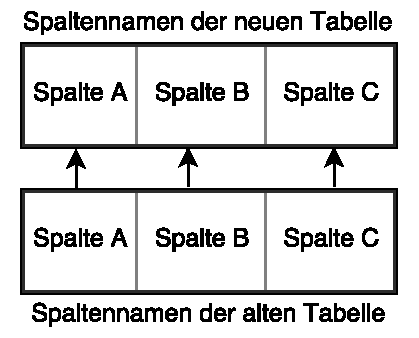
\includegraphics[width=0.5\textwidth]{images/hash_new.pdf}}
        \centering
        \caption{Die Darstellung der Spaltenzuordnung durch einen Hash}
        \label{pic:hash_new}
\end{figure}

\begin{figure}[ht]
  \begin{subfigure}[b]{0.45\textwidth}
    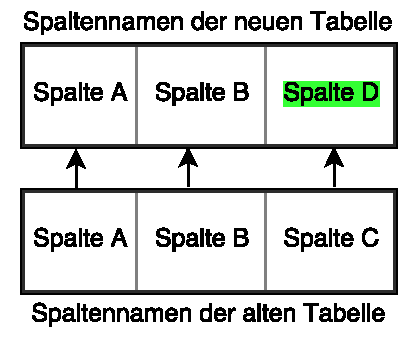
\includegraphics[width=\textwidth]{images/hash_rename.pdf}
    \caption{Umbenennen einer Spalte}
    \label{fig:hash_rename}
  \end{subfigure}\hfill
  \begin{subfigure}[b]{0.45\textwidth}
    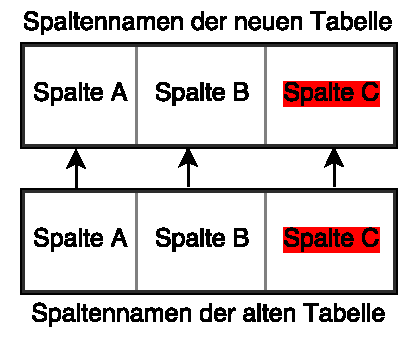
\includegraphics[width=\textwidth]{images/hash_remove.pdf}
    \caption{Entfernen einer Spalte}
    \label{fig:hash_remove}
  \end{subfigure}
  \caption{Hash - Entfernen \& Umbenennen einer Spalte}
  \label{fig:hash_remove_rename}
\end{figure}

\item[Änderungen einzeln oder alle durchführen] \hfill\\
Mit der jetzigen Implementierung wird jede Änderung einzeln an der Datenbank durchgeführt. Durch die Implementierung des Hashs für die Spaltenzuweisung und der Abbildung der Tabelle auf dem Server, könnten alle Änderung auf dem Server durchgeführt werden, bevor diese an die Datenbank weitergeleitet werden. Dies würde die Zugriffe auf die Datenbank deutlich verringern, und somit die Synchronisierung auf die Datenbankzugriffe von verschiedenen Benutzern vereinfachen. Der Nachteil wäre, dass nicht festzustellen ist, welche Veränderung gegebenenfalls fehlgeschlagen ist. Da die Zielgruppe Anfänger im Thema Datenbanken ist, ist die Fehlerkommunikation ein wichtigerer Aspekt, der einen Vorrang hat.  

\item[Sicherung der Datenbank] \hfill\\
Bei der Veränderung der Datenbank in Einzelschritten, schlagen Veränderungen innerhalb der Kette von Veränderungen fehl, nachdem einige Änderungen bereits an der Datenbank durchgeführt wurden. Dabei muss die Datenbank beim Fehlschlagen der Veränderungskette auf den ursprünglichen Zustand zurückgeführt werden. In SQLite werden, anders als in anderen Datenbanksystemen, Verschachtelungen von Transaktionen nicht unterstützt. Dafür wird in SQLite eine Datenbank in einer einzelnen Datei gespeichert. \\ 
Es kann damit eine Kopie dieser Datei beim Anfang der Migration erstellt werden, um diese gegebenenfalls wiederherzustellen.

\end{description}

\subsubsection{Tests}
\label{subsubsec04:server_testing}
Um die einzelnen Funktionen zu testen, wurden die bereits von Marcus Riemer genutzten Möglichkeiten verwendet, um Unit-Tests zu schreiben. \\
Damit konnte sichergestellt werden, dass Funktionen sich in der Weise verhalten haben wie es erwartet war. Diese Tests waren die einzige Möglichkeit die Funktionalität zu testen, die nicht direkt per Oberfläche gesteuert werden konnten. Wie bereits in~\ref{fk_disclaimer} erwähnt, wurde keine Lösung gefunden für die Darstellung von zusammengesetzten Foreign Keys. Mit Tests wurde sichergestellt, dass der Server auch diese unterstützt, damit in Zukunft zusammengesetzte Foreign Keys im Client eingebaut werden können.

\subsubsection{Unerwartete Probleme}
\label{subsubsec04:server_problems}

Während der Entwicklung auf dem Server sind einige Schwierigkeiten aufgetreten, so muss unter anderem die \texttt{REGEXP}-Funktion bei jeder Verbindung mit der Datenbank definiert werden und das größte Problem lag in der Nutzung von \texttt{PRAGMA}-Funktionen.

\begin{description}
\item[PRAGMA foreign\_key\_check löst SQLException aus] \hfill\\
In dem Algorithmus zum Verändern der Tabelle wird die Konsistenz der Datenbank mit dem Befehl ``PRAGMA foreign\_key\_check'' geprüft. (Schritt 12:~\ref{enum:sql_algo}) \\
Das \texttt{PRAGMA} gibt eine Tabelle zurück, mit Einträgen die anzeigen welche Tabelle und welche Spalte die Konsistenz verletzen. 
Sollte die Datenbank inkonsistent sein, wird eine SQLException geworfen und in der Message der Exception ist die Tabelle mit den Einträgen enthalten. Die Exception vom Typ SQLException, wird bei den meisten Fehlern geworfen die mit SQL verbunden sind. Dies ist ein Problem, wenn alle geworfenen Fehler als Ergebnis der Konsistenzprüfung interpretiert werden. Aus diesem Grund musste die Prüfung in eine separate Funktion ausgelagert werden. \\
Ab der SQLite Version 3.16.0 die am 2. Januar 2017 erschienen ist, lassen sich \texttt{PRAGMA}-Funktionen, die eine Ausgabe liefern, innerhalb von \texttt{SELECT}-Statements benutzen. Diese werden als Tabellen interpretiert und sind erreichbar über den Funktionsnamen mit dem Präfix ``pragma\_''. Damit lässt sich das Auslösen einer SQLException mit dem Aufruf \texttt{SELECT * from pragma\_foreign\_key\_check} verhindern. Diese sehr junge Erweiterung, war auf der Entwicklermaschine noch nicht vorhanden, und ist nicht auf dem zukünftigen Server garantiert vorhanden, was dazu führt, dass vorerst die Implementierung per \texttt{PRAGMA}-Funktionen verwendet wird.
\end{description}
